%\documentclass[border={0.1cm 0.1cm 0.1cm 0.1cm}]{standalone}  %E,S,W,N
\documentclass{scrartcl}

\usepackage{amssymb}
\usepackage{amsmath}
\usepackage{tikz}

\begin{document}
	
	\hspace{-2cm}%
	\scalebox{0.5}{
	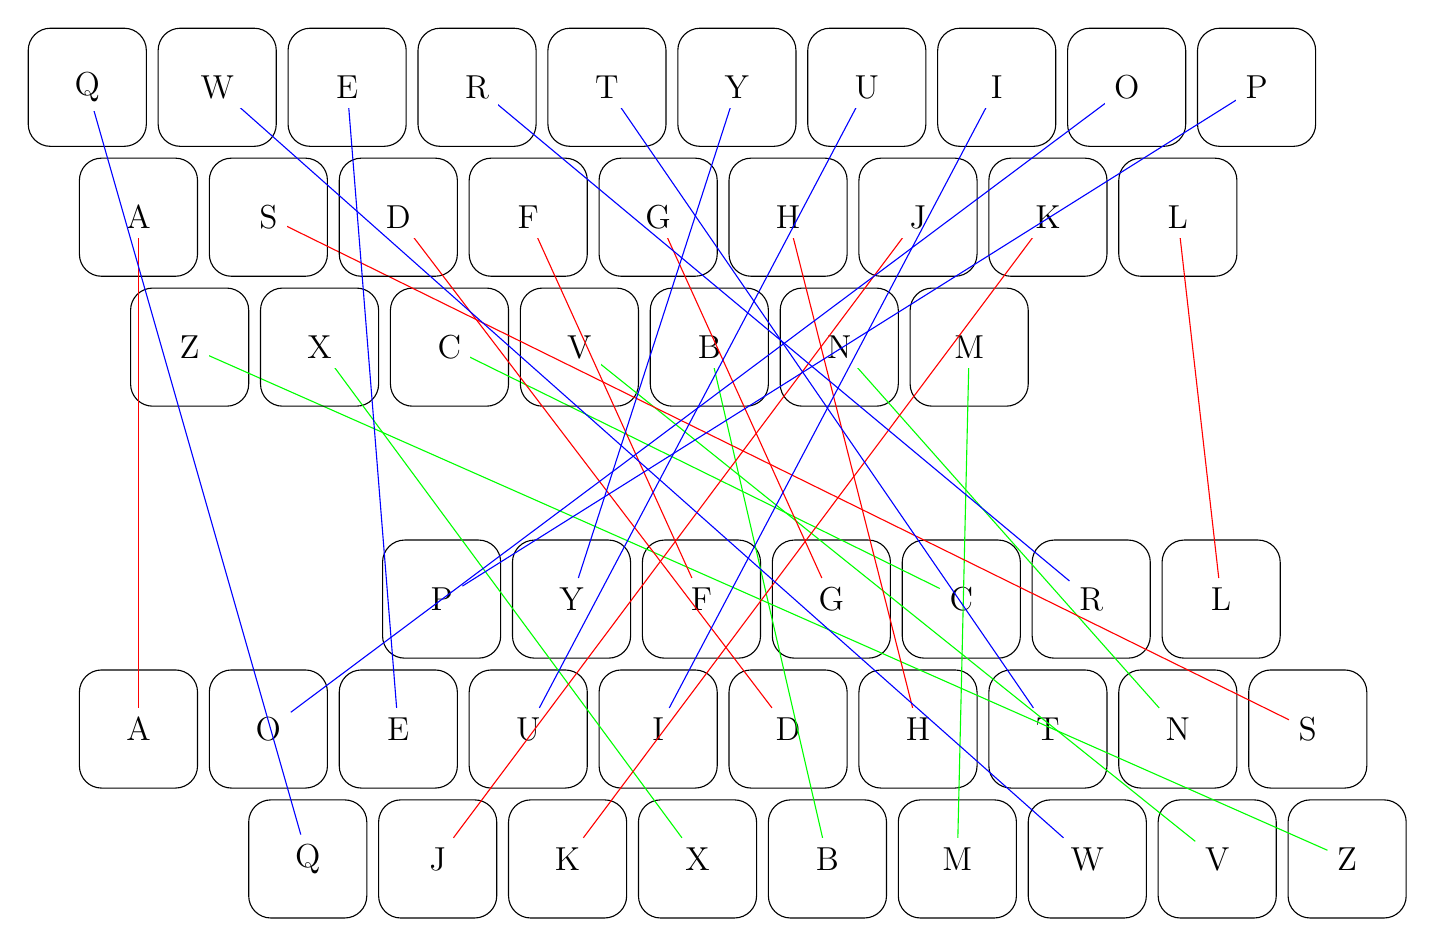
\begin{tikzpicture}	
	\def\s{0.75} %side length for keys
	\def\d{0.15} %distance between keys
	
	%DVORAK -- goes first due to qwerty-centric line colors: need to define (\i) nodes first
	\foreach \i [count=\j] in {P,Y,F,G,C,R,L}{ 
		\draw[rounded corners=8pt,yshift=-6.5cm] ({6*\s+(2*\s+\d)*\j-\s},-\s) rectangle ++(2*\s,2*\s);
		\node[yshift=-6.5cm] (\i) at ({6*\s+(2*\s+\d)*\j},0) {\large\i};
	}
	\foreach \i [count=\j] in {A,O,E,U,I,D,H,T,N,S}{ 
		\draw[rounded corners=8pt,yshift=-6.5cm] ({0.65+(2*\s+\d)*\j-\s},-3*\s-\d) rectangle ++(2*\s,2*\s);
		\node[yshift=-6.5cm] (\i) at ({0.65+(2*\s+\d)*\j},-2*\s-\d) {\large\i};
	}
	\foreach \i [count=\j] in {Q,J,K,X,B,M,W,V,Z}{ 
		\draw[rounded corners=8pt,yshift=-6.5cm] ({2*\s+1.3+(2*\s+\d)*\j-\s},-5*\s-2*\d) rectangle ++(2*\s,2*\s);
		\node[yshift=-6.5cm] (\i) at ({2*\s+1.3+(2*\s+\d)*\j},-4*\s-2*\d) {\large\i};
	}
	
	%QWERTY -- reverse order for rows because of fill=white
	\foreach \i [count=\j] in {Z,X,C,V,B,N,M}{ 
		\draw[rounded corners=8pt] ({1.3+(2*\s+\d)*\j-\s},-5*\s-2*\d) rectangle ++(2*\s,2*\s);
		\draw[green] ({1.3+(2*\s+\d)*\j},-4*\s-2*\d)--(\i);
		\node[fill=white] at ({1.3+(2*\s+\d)*\j},-4*\s-2*\d) {\large\i};
	}
	\foreach \i [count=\j] in {A,S,D,F,G,H,J,K,L}{ 
		\draw[rounded corners=8pt] ({0.65+(2*\s+\d)*\j-\s},-3*\s-\d) rectangle ++(2*\s,2*\s);
		\draw[red] ({0.65+(2*\s+\d)*\j},-2*\s-\d)--(\i);
		\node[fill=white] at ({0.65+(2*\s+\d)*\j},-2*\s-\d) {\large\i};
	}
	\foreach \i [count=\j] in {Q,W,E,R,T,Y,U,I,O,P}{ 
		\draw[rounded corners=8pt] ({(2*\s+\d)*\j-\s},-\s) rectangle ++(2*\s,2*\s);
		\draw[blue] ({(2*\s+\d)*\j},0)--(\i);
		\node[fill=white] at ({(2*\s+\d)*\j},0) {\large\i};
	}
	\end{tikzpicture}%
	%
	\hspace{0.25cm}%
	%
	%
	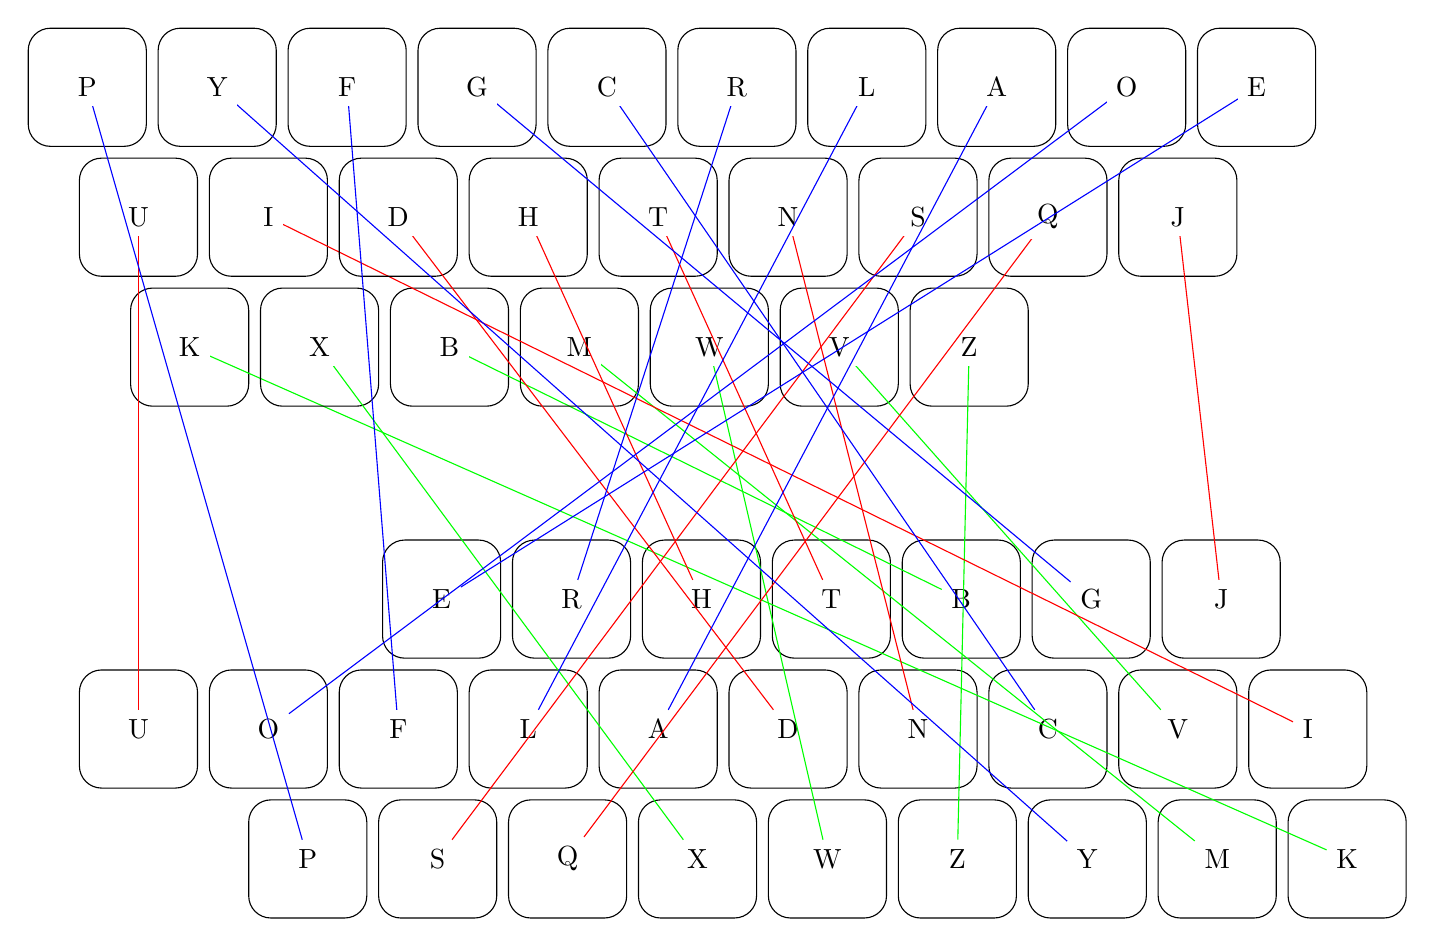
\begin{tikzpicture}	
	\def\s{0.75} %side length for keys
	\def\d{0.15} %distance between keys
	
	%DVORAK -- goes first due to qwerty-centric line colors: need to define (\i) nodes first
	\foreach \i [count=\j] in {E,R,H,T,B,G,J}{ 
		\draw[rounded corners=8pt,yshift=-6.5cm] ({6*\s+(2*\s+\d)*\j-\s},-\s) rectangle ++(2*\s,2*\s);
		\node[yshift=-6.5cm] (\i) at ({6*\s+(2*\s+\d)*\j},0) {\i};
	}
	\foreach \i [count=\j] in {U,O,F,L,A,D,N,C,V,I}{ 
		\draw[rounded corners=8pt,yshift=-6.5cm] ({0.65+(2*\s+\d)*\j-\s},-3*\s-\d) rectangle ++(2*\s,2*\s);
		\node[yshift=-6.5cm] (\i) at ({0.65+(2*\s+\d)*\j},-2*\s-\d) {\i};
	}
	\foreach \i [count=\j] in {P,S,Q,X,W,Z,Y,M,K}{ 
		\draw[rounded corners=8pt,yshift=-6.5cm] ({2*\s+1.3+(2*\s+\d)*\j-\s},-5*\s-2*\d) rectangle ++(2*\s,2*\s);
		\node[yshift=-6.5cm] (\i) at ({2*\s+1.3+(2*\s+\d)*\j},-4*\s-2*\d) {\i};
	}
	
	%QWERTY -- reverse order for rows because of fill=white
	\foreach \i [count=\j] in {K,X,B,M,W,V,Z}{ 
		\draw[rounded corners=8pt] ({1.3+(2*\s+\d)*\j-\s},-5*\s-2*\d) rectangle ++(2*\s,2*\s);
		\draw[green] ({1.3+(2*\s+\d)*\j},-4*\s-2*\d)--(\i);
		\node[fill=white] at ({1.3+(2*\s+\d)*\j},-4*\s-2*\d) {\i};
	}
	\foreach \i [count=\j] in {U,I,D,H,T,N,S,Q,J}{ 
		\draw[rounded corners=8pt] ({0.65+(2*\s+\d)*\j-\s},-3*\s-\d) rectangle ++(2*\s,2*\s);
		\draw[red] ({0.65+(2*\s+\d)*\j},-2*\s-\d)--(\i);
		\node[fill=white] at ({0.65+(2*\s+\d)*\j},-2*\s-\d) {\i};
	}
	\foreach \i [count=\j] in {P,Y,F,G,C,R,L,A,O,E}{ 
		\draw[rounded corners=8pt] ({(2*\s+\d)*\j-\s},-\s) rectangle ++(2*\s,2*\s);
		\draw[blue] ({(2*\s+\d)*\j},0)--(\i);
		\node[fill=white] at ({(2*\s+\d)*\j},0) {\i};
	}
	\end{tikzpicture}
	} %end scalebox
	
\end{document}